% !TeX spellcheck = en_US
 \documentclass[AIRbeamer
               ,optEnglish
               %,handout%               deactivate animation
               ,optBiber
               ,optBibstyleAlphabetic
               ,optBeamerClassicFormat% 4:3 format
               %,optBeamerWideFormat%   16:9 format
               ]{AIRlatex}

%\setbeameroption{show notes}

\graphicspath{{figures/}}%
\addbibresource{source/literature.bib}%

\title[Active Tactile Exploration Based on Whisker-Inspired Sensory Array]{Active Tactile Exploration Based on Whisker-Inspired Sensory Array}
\def\PresentationType{\AIRlangGerEng{Abschlussvortrag}{Final Presentation}}
\def\PresentationThesisType{\AIRlangBachelorsThesis}
\author[Valentin Safronov]{Valentin Safronov}
\def\PresentationExaminer{\AIRnamesProfKnoll}
\def\PresentationSupervisor{Yixuan Dang, M.Sc.}
\date{\AIRutilsDate{28}{03}{2025}}

\AIRbeamerSetupHeader{\AIRlayoutHeaderCustomChair}
\AIRbeamerSetupFooterCD

\begin{document}
\AIRbeamerTitlePageStudentThesis

\begin{frame}{Outline}
  \tableofcontents
\end{frame}


\section{Motivation}

\subsection{Biological Whisker Structure}

\subsection{Robotic Whisker Sensors}


\section{Related Work}

\section{Hardware}

\subsection{Single Whisker}

\begin{frame}[c]{Single Whisker Sensor}
\centering
\begin{columns}[c,onlytextwidth]
  \column{0.3\textwidth}
    \centering
    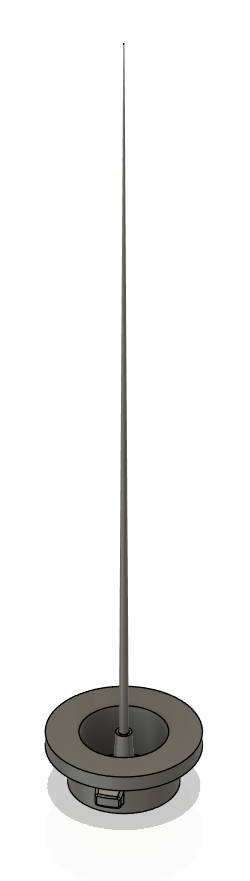
\includegraphics[height=0.6\textheight]{figures/whisker}\\
    (a) Whisker Sensor,\\Whisker shaft -- a nitinol wire
  \column{0.3\textwidth}
    \centering
    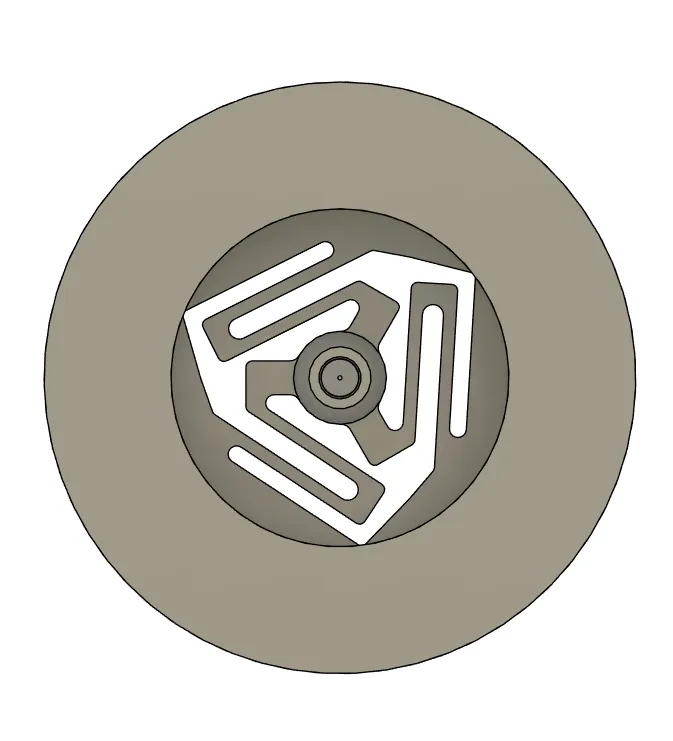
\includegraphics[height=0.6\textheight]{figures/suspension}\\
    (b) Suspension,\\3D-printed with PLA
  \column{0.3\textwidth}
    \centering
    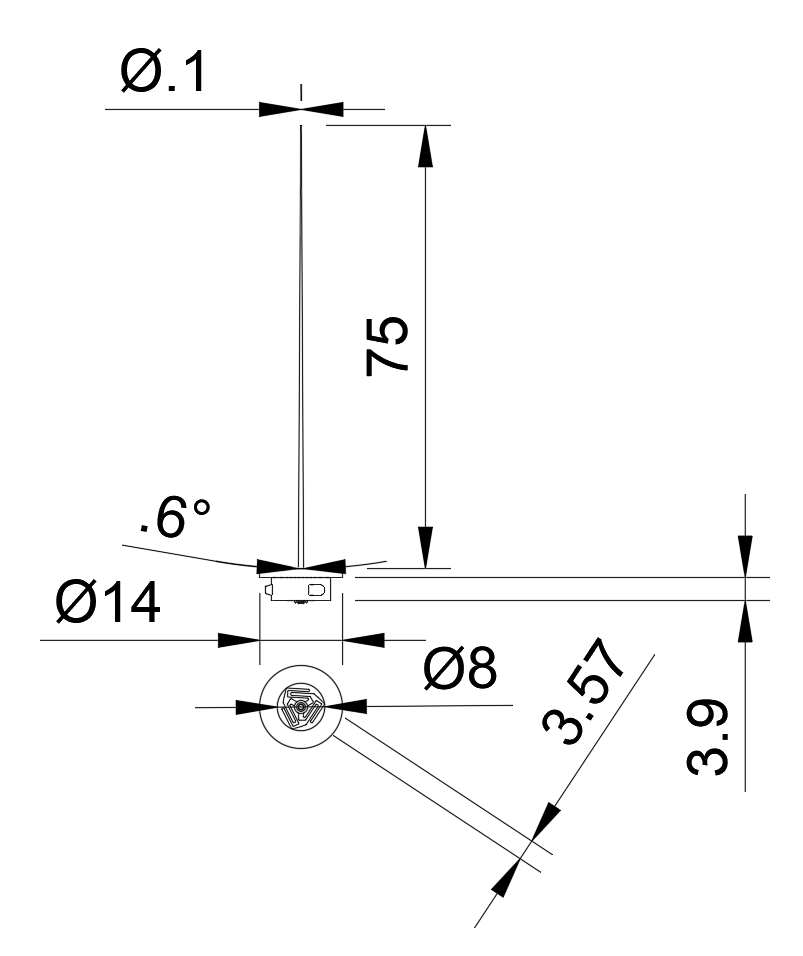
\includegraphics[height=0.6\textheight]{figures/whisker-dims}\\
    (c) Whisker sensor dimensions
\end{columns}
\end{frame}

\note[itemize]{
    \item The whisker shaft is first glued to the suspension system.
    \item A neodymium permanent magnet, axially magnetized with its field direction aligned with the wire, is placed underneath.
    \item The suspension hooks are designed to allow screwing in the whiskers into the whisker mount.
}

\subsection{Whisker Array Platform}
\subsection{Data Acquisition}


\section{Control Policies and Results}
\subsection{Swiping Policy}
\subsection{Retrieval Policy}
\subsection{Tunneling Policy}


\section{Infrastructure}
\section{Future Work}
\section{Conclusion}


\AIRbeamerSetFooterText{References}%
\begin{frame}[allowframebreaks]{References}%
    %\sloppy% "Word"-like typesetting in order to improve breaking lines with long URLs/DOIs
    \printbibliography[heading=none]%
\end{frame}%

\AIRbeamerTitlePageStudentThesis%

\end{document}%
